% !TEX encoding = UTF-8 Unicode

\documentclass[twocolumn,10pt,a4j]{ltjsarticle}
\usepackage{kougai}

\title{個人でのVR技術の利用状況}
\author{1932131 三原 巧巳  指導教員 須田 宇宙 准教授}
\date{}

\begin{document}

\maketitle

\section{はじめに}
近年,xR(AR,MR,VR)技術の発展やコンテンツが増えたことにより,私たちの日常生活の中でも見かける機会も増えている.
現在,AR技術とMR技術を利用するにはスマートフォンやスマートグラスなどが用いられ,技術を利用するにはスペースをあまり必要としていないことが多い.
AR技術はスマートフォンを利用したコンテンツが多く存在し,MR技術は工業や医療の場で多く利用される.

一方,VR技術は機材の出荷台数が年々増えており,今後も増えていくと予想がされているが日常生活で見かけることが少ない\cite{VRの機材の出荷台数}.
利用するには,ヘッドマウントディスプレイを装着した上で動き回るため,コンテンツによっては大きな機材や広い場所も必要となる.
VR技術は,ゲームやアトラクション施設の場で利用されることが多いが数は少ないというところが問題である.
これからも普及率が低い場合VR技術が発展していかなくなってしまいエンターテイメントの幅が広がらないだけではなく,現実では危険な実習や現実には起こしづらい現象の体験が困難である.

本研究では,普及しない理由はコンテンツにあると仮説を立て,それを元にVR機器の普及度と,購入されている種類・傾向,および購入していない人に対して,購入していない理由などについて調査をすることを目的としている.

\section{xRについて}
AR(Augmented Reality:拡張現実)とは,カメラで現実世界を映し,その上にCG映像や文字情報を重ねる技術である.
%ARコンテンツを利用するためには,専用の機材を必要とせず携帯端末などで利用することができる.

MR(Mixed Reality:複合現実)とは,カメラを通して現実世界を認識し,実写とCG映像や文字情報を重ねることで現実世界と仮想世界を融合させる技術である.
%MR技術を利用するには,専用のデバイスやカメラだけではなく,仮想世界で作られたものを映すためのマーカーなども必要となる.

VR(Virtual Reality:仮想現実)とは,専用のゴーグルを装着して,視界全体に映像を映すことで映像の中に入り込んだような体験ができる技術である.
さらにVRの中で移動や物体の操作などができ,現実に近い体験から非現実的な体験まで幅広く扱うことができる.
%VRコンテンツを利用するためには,専用のゴーグルと専用のコントローラーなどが必要となる.

%図1に示すように2021年ではVRを認知している人は90%もいるが,実際に利用したことある人は全体の17%のみであり,継続して利用していたのは5%という結果からVR技術はあまり普及していない[1].

%\begin{figure}[h]
%\begin{center}
% 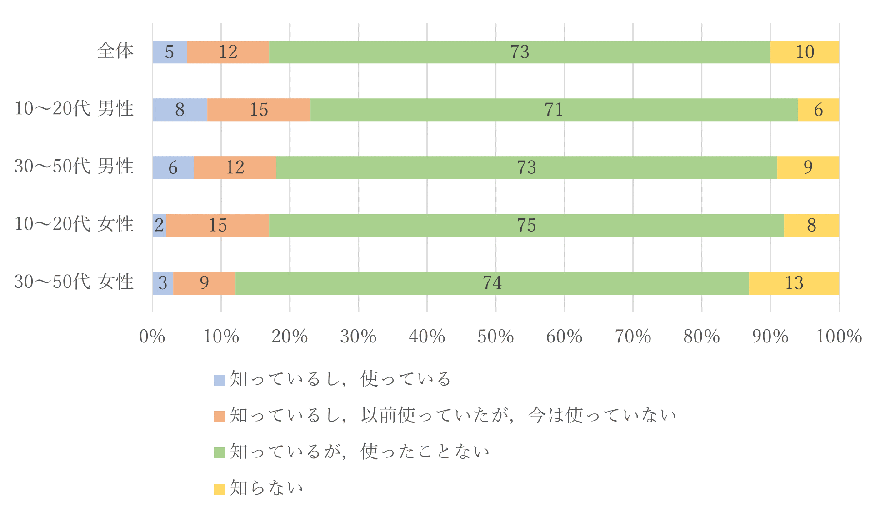
\includegraphics[clip,width=85mm,height=55mm]{グラフ_0903.pdf}
%\end{center}
% \caption{VRの現状}
% \label{fig:比較グラフ}
%\end{figure}


\section{調査について}
現在,VR機材には高い機器もありその機器を利用したコンテンツもあるが,ほかのゲーム機器やスマートフォンなどと比べると金額の差はさほどない.
VRコンテンツが普及しない理由として長期間かつ多くの人に人気になるようなコンテンツがないという仮説を立てた.

本研究では,アンケート2回行った.
1回目のアンケートでは,VRの体験をしたことがあるかの有無と,VR機器の所持/非所持で分け,VRに求められているコンテンツや購入目的などを調査した.
2回目のアンケートでは,主に機材と普及度を向上させるコンテンツについて調査した.
アンケートは,いずれもGoogle Formsを使用し,本学学生を対象者とした.

図\ref{fig:vr機器を所持するまでに至らなかった理由.pdf},\ref{fig:購入したいと考えたvrコンテンツ.pdf}は調査結果の一部である.
図\ref{fig:vr機器を所持するまでに至らなかった理由.pdf}はVR機器を購入していない人に対する購入に至らなかった理由の集計結果であり,機材の価格が高いという回答が多かった.
図\ref{fig:購入したいと考えたvrコンテンツ.pdf}の調査はVRに求められるコンテンツの集計結果であり,Zenith: The Last Cityとアフェクテッド恐怖の館はVRのみのコンテンツである.
バイオハザード4VRとAmong Us VRはVRを用いてないコンテンツの人気作品として今回取り上げた.
調査結果から有名タイトルのVR化よりVRを感じやすいコンテンツが求められていることが分かった.

\begin{figure}[h]
\begin{center}
 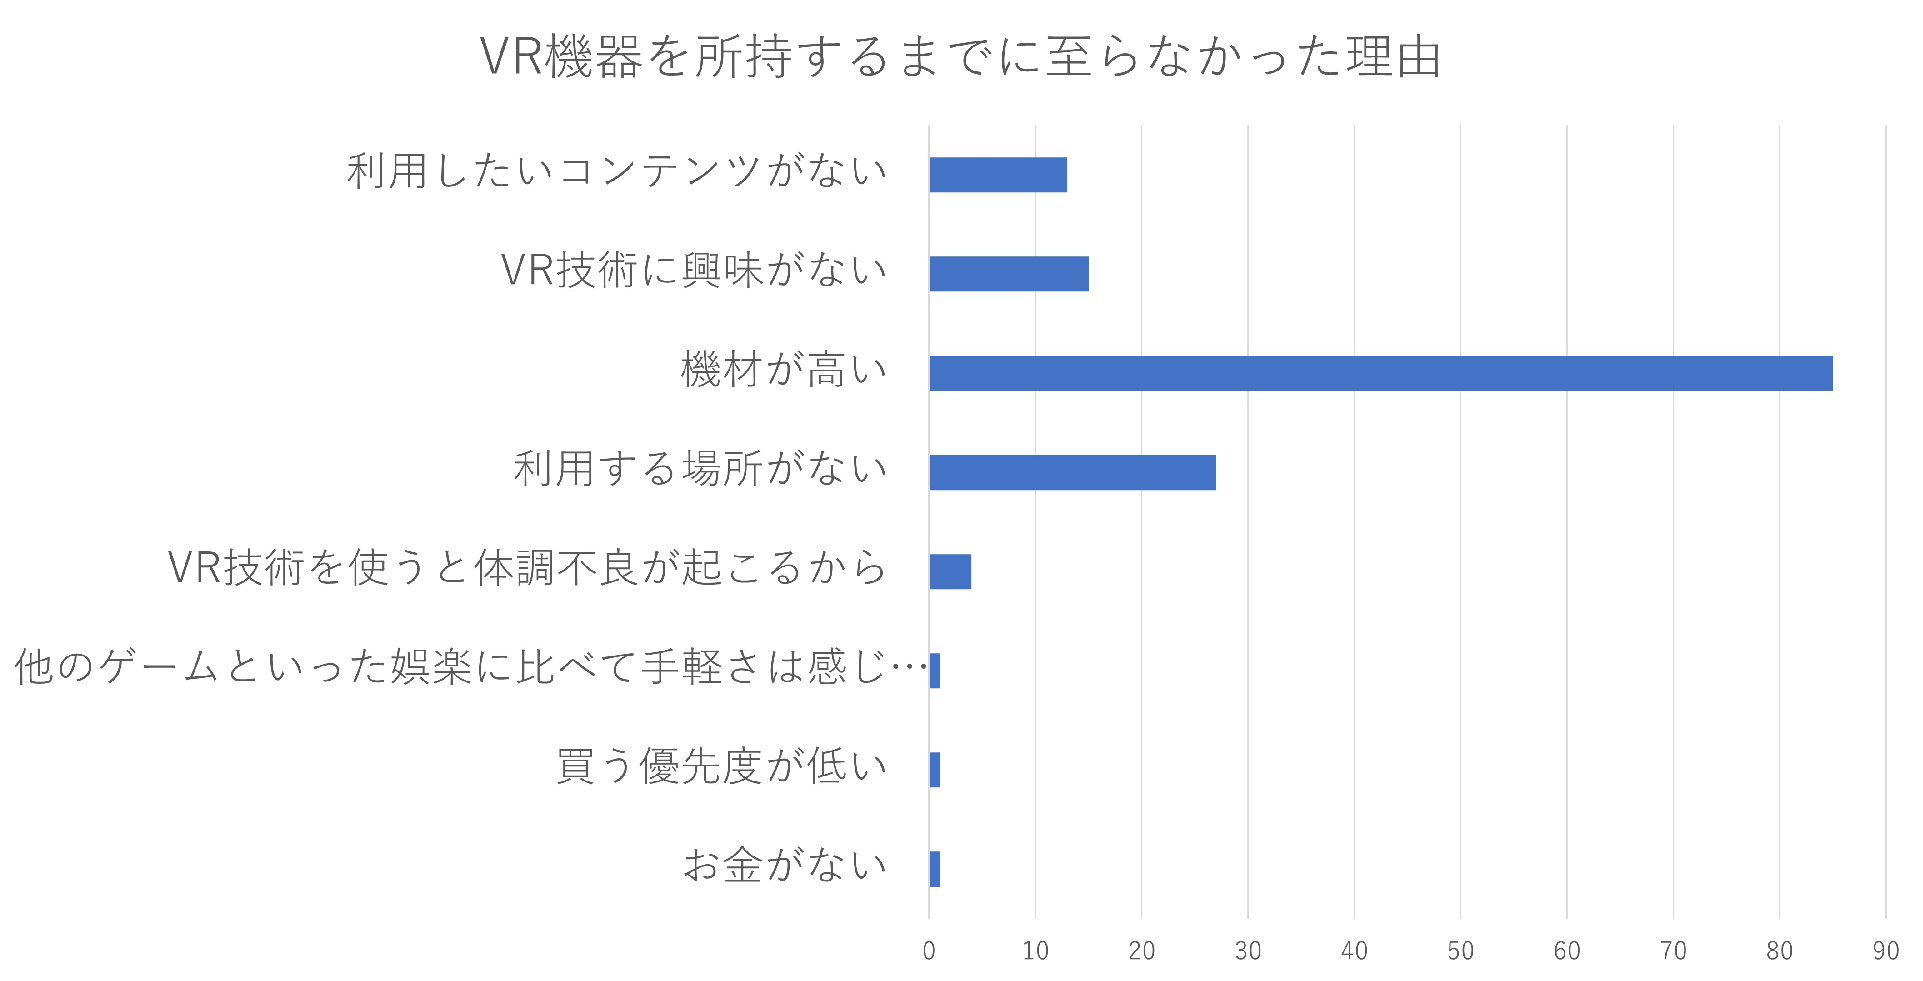
\includegraphics[clip,width=85mm,height=30mm]{vr機器を所持するまでに至らなかった理由.pdf}
\end{center}
 \caption{VR機器を購入するに至らなかった理由の調査結果}
 \label{fig:vr機器を所持するまでに至らなかった理由.pdf}
\end{figure}
\vspace{2mm}

\begin{figure}[h]
\begin{center}
 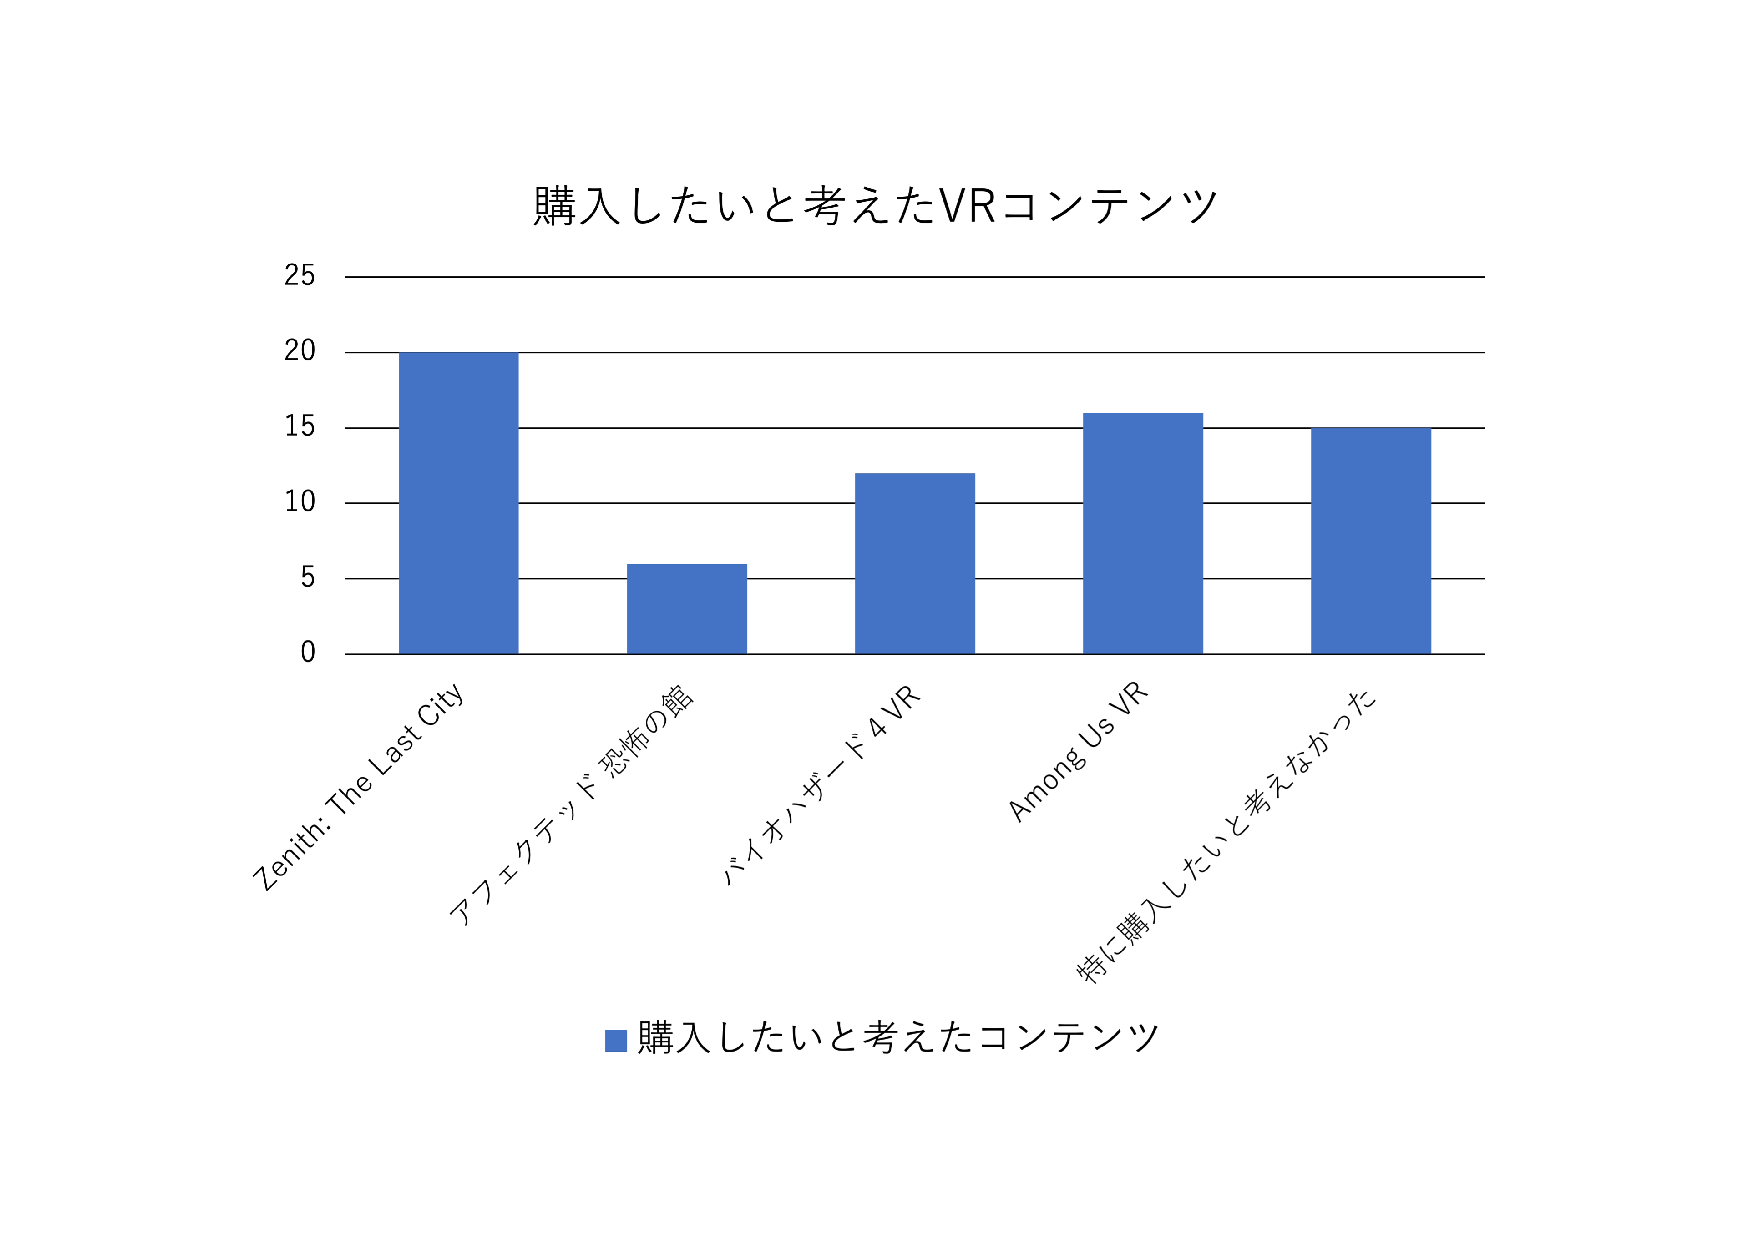
\includegraphics[clip,width=85mm,height=55mm]{購入したいと考えたvrコンテンツ.pdf}
\end{center}
 \caption{VRに求められるコンテンツの調査結果}
 \label{fig:購入したいと考えたvrコンテンツ.pdf}
\end{figure}

%今回のアンケートの作成したには,Google Fprmsを使用し,アンケートの対象として千葉工業大学の学生を対象とした.

\section{おわりに}
本研究では,VR機器が普及しない理由がコンテンツであると仮説を立てアンケート調査を行った.
その結果からコンテンツは十分であり,機材のコストが障壁になっていることが分かった.

\begin{thebibliography}{99}
%\bibitem{VR}  ``流行体感から読み解くサービス未来予測 流行予想シリーズ ~VR(バーチャルリアリティ)編~'', \url{https://research-platform.line.me/archives/38203466.html}, 2022/9/2参照

\bibitem{VRの機材の出荷台数}  ``2021年、VR/ARヘッドセット出荷台数は1,000万台に迫った――IDCが発表
'', \url{https://moguravr.com/idc-vr-ar-headset-market-overview/}, 2023/1/13参照

\end{thebibliography}

\end{document}
